\documentclass[10pt, compress, aspectratio=169]{beamer}

\usetheme[numbering=fraction, progressbar=none, titleformat=smallcaps]{metropolis}
\usepackage{booktabs}
\usepackage{array}
\usepackage{listings}
\usepackage{graphicx}
\usepackage[scale=2]{ccicons}
\usepackage{url}
\usepackage{relsize}
\usepackage{wasysym}

\usepackage{pgfplots}
\usepgfplotslibrary{dateplot}

\lstset{ %
  backgroundcolor={},
  basicstyle=\ttfamily\footnotesize,
  breakatwhitespace=true,
  breaklines=true,
  captionpos=n,
  commentstyle=\color{orange},
  escapeinside={\%*}{*)},
  extendedchars=true,
  frame=n,
  keywordstyle=\color{orange},
  language=C++,
  rulecolor=\color{black},
  showspaces=false,
  showstringspaces=false,
  showtabs=false,
  stepnumber=2,
  stringstyle=\color{gray},
  tabsize=2,
  keywords={thrust,plus,device_vector, copy,transform,begin,end, copyin,
  copyout, acc, \_\_global\_\_, void, int, float, main, threadIdx, blockIdx,
  blockDim, if, else, malloc, NULL, cudaMalloc, cudaMemcpy, cudaSuccess,
  cudaGetLastError, cudaDeviceSynchronize, cudaFree, cudaMemcpyDeviceToHost,
  cudaMemcpyHostToDevice, const, data, independent, kernels, loop,
  fprintf, stderr, cudaGetErrorString, EXIT_FAILURE, for, dim3},
  otherkeywords={::, \#pragma, \#include, <<<,>>>, \&, \*, +, -, /, [, ], >, <}
}

\renewcommand*{\UrlFont}{\ttfamily\smaller\relax}

\graphicspath{{images/}}

\title{Capability}
\author{\footnotesize Rodrigo Siqueira \\ {\scriptsize siqueira@ime.usp.br}}
\institute{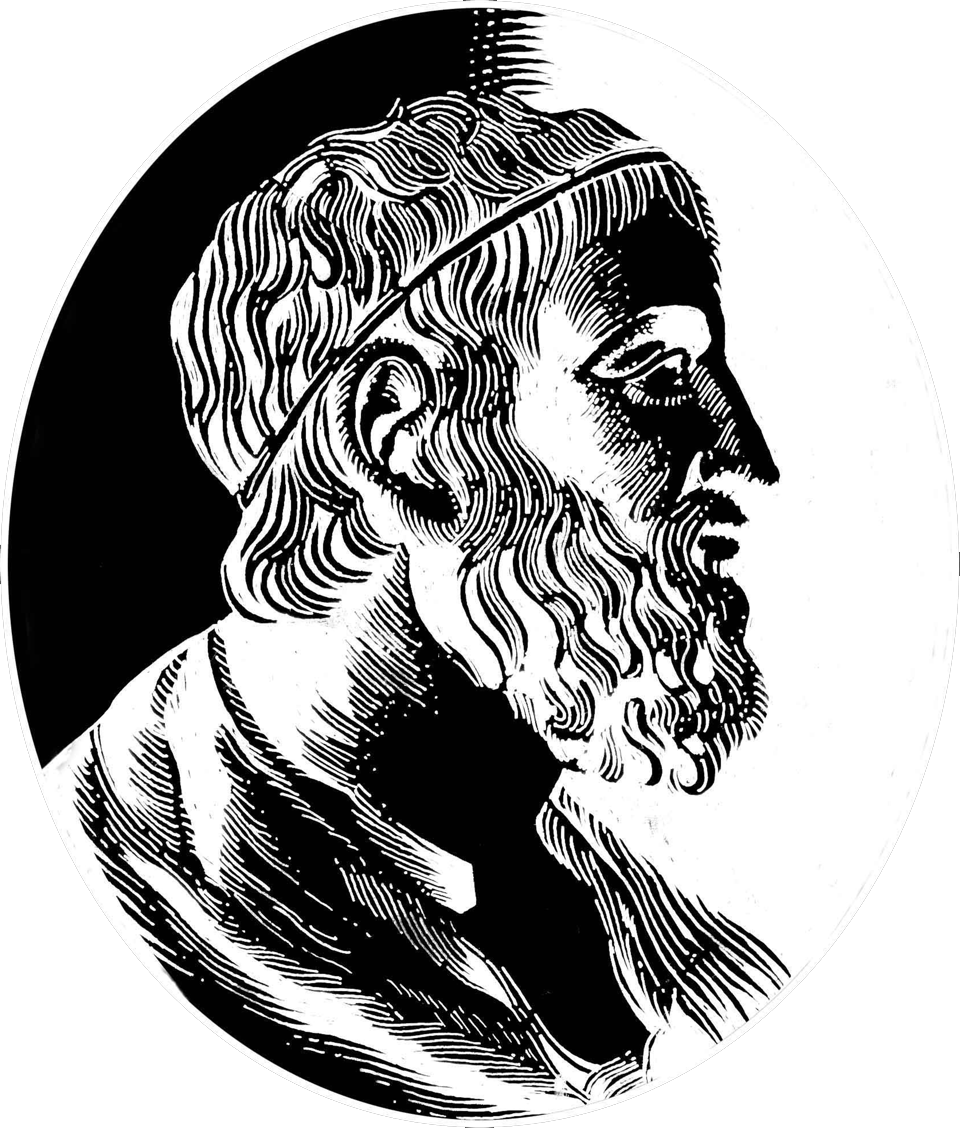
\includegraphics[height=2cm]{imelogo}\\[0.2cm] Department of Computer Science \\ University of São Paulo}

\begin{document}

\maketitle

%------------------------------------------------------------------------------
\section{Introduction}
\begin{frame}{Problem}
  \begin{itemize}
    \item It is hard to share information between process
    \item Protection and safety of objects
    \item Reliable construction
  \end{itemize}
\end{frame}

%------------------------------------------------------------------------------
\section{Capability (CB)}
\begin{frame}{Overview}
  \begin{itemize}
    \item Access by token
    \item Data structure with:
    \begin{itemize}
      \item Unique identify of object
      \item Access right
    \end{itemize}
    \item Mechanisms
    \begin{itemize}
      \item Unique memory address
      \item Unique way to address software and hardware
    \end{itemize}
    \item Capability list
  \end{itemize}
\end{frame}

\begin{frame}{Capability (CB) - Operations}
  \begin{itemize}
    \item Move capability inside list
    \item Remove capability
    \item Restrict permission
    \item Pass capability as a parameters
    \item Transmit capability to other users
  \end{itemize}
\end{frame}

%------------------------------------------------------------------------------
\section{Memory address}
\begin{frame}{Memory Address}
  \begin{itemize}
    \item Each process has a capability list, which define the access segment
    \item Memory address with capability
    \item Hardware instructions to transfer CB
    \item CB register Vs CB list
  \end{itemize}
\end{frame}

\begin{frame}{Memory address properties}
  \begin{itemize}
    \item Virtual address space segmented
    \item Control the bit patterns
    \item Dynamic change of Address Space
    \item Virtual Address space identify local process
    \item Context independent
  \end{itemize}
  \begin{itemize}
    \item Process can only affect objects in which CB was loaded
    \item Just access the required segment
    \item It is easy to determine the segment
  \end{itemize}
\end{frame}

%------------------------------------------------------------------------------
\section{Address context}
\begin{frame}{Address context}
  \begin{itemize}
    \item Each object has a unique identify
    \item Hardware uses fields to locale object
    \item Address are independent of context
    \item Larger identifiers
    \item long-term Vs Short-term
  \end{itemize}
\end{frame}

%------------------------------------------------------------------------------
\section{Security}
\begin{frame}{An example from real life}
  % TODO: Put a table example
  
\end{frame}
\end{document}
